\newpage
IRSTI 50.41.25;50.47.31

\sectionwithauthors{K. Akishev, K.Aryngazin, B.Biybosynov}{THE USE OF INFORMATION TECHNOLOGIES IN CALCULATING THE
PRODUCTIVITY OF TECHNOLOGICAL EQUIPMENT FOR THE PRODUCTION OF CERAMIC PRODUCTS BASED ON MAN-MADE RAW MATERIALS}

\begin{center}
{\bfseries \textsuperscript{1}K. Akishev\envelope,
\textsuperscript{2}K.Aryngazin, \textsuperscript{3}B.Biybosynov}

\textsuperscript{1}Kazakh University of Technology and Business named
after K.Kulazhanov, Astana, Kazakhstan,

\textsuperscript{2}"EcostroyNII-PV" LLP, Pavlodar, Kazakhstan\emph{,}

\textsuperscript{3}Kyrgyz State University named after I. Arabaev
\end{center}
\envelope Corresponding author: Akmail04cx@mail.ru \vspace{0.5cm}

Currently, a large amount of man-made waste has been stored on the
territory of the Republic of Kazakhstan, which, by their chemical and
mineral properties, are a serious raw material base for the production
of building materials.

The quality indicators of raw materials affect not only the physical and
strength characteristics of the finished product, but also the cost. In
our study, we use man-made raw materials for the production of
construction products, as additives to clay for the semi-dry method of
producing ceramic products, since this method is less labor-intensive
and does not require large financial investments. One of the most
important characteristics of technological equipment is performance.
Technological equipment for the production of construction products is
represented on the market of Kazakhstan by leading foreign companies,
including Chinese, Russian, Turkish, Spanish, Kazakh manufacturers are
not included in this list. Technological equipment can produce products
from a certain type of raw materials, for which such parameters as
productivity, quality indicators of raw materials and others are
indicated in the technical documentation. That is, when using
technogenic raw materials as additives to the charge, it is not possible
to determine productivity, for objective reasons. In this regard, the
task of calculating the productivity of the technological line for the
production of ceramic products using information technology is relevant.

As a software tool in the study, the program "Simulation model of a
technological line for the production of construction products using
industrial waste" is used, written in C++, in accordance with the
principles of object-oriented programming. Performance calculations were
performed for technological equipment Titanium 900-120 DHEX press,
Titanium 80 D press. The presented program can be used by individual
entrepreneurs not only to calculate productivity, output volume, but
also to justify the choice of technologi-cal equipment for the production
of ceramic products.

{\bfseries Keywords:} modeling, information technology, programming
language, program, technological \\equipment, productivity, ceramic
products.


\sectionheading{ТЕХНОГЕНДІК ШИКІЗАТ НЕГІЗІНДЕ КЕРАМИКАЛЫҚ БҰЙЫМДАР ӨНДІРІСІНІҢ ТЕХНОЛОГИЯЛЫҚ ЖАБДЫҒЫНЫҢ ӨНІМДІЛІГІН ЕСЕПТЕУ КЕЗІНДЕ АҚПАРАТТЫҚ ТЕХНОЛОГИЯЛАРДЫ ПАЙДАЛАНУ}
\begin{center}
{\bfseries \textsuperscript{1}K.Акишев\envelope,
\textsuperscript{2}K. Арынгазин, \textsuperscript{3}Б.Бийбосынов}

\textsuperscript{1}Қ.Құлажанов атындағы Қазақ технология және бизнес
университеті АҚ, Астана, Қазақстан,

\textsuperscript{2}"ЭкостройНИИ-ПВ" ЖШС директоры, Павлодар қ.,
Қазақстан,

\textsuperscript{3}И. Арабаев атындағы Қырғыз мемлекеттік университеті,
Қырғызстан,

e-mail:Akmail04cx@mail.ru
\end{center}

Қазіргі уақытта Қазақстан Республикасының аумағында өзінің
химиялық-минералды қасиеттері бойынша құрылыс материалдарын өндіру үшін
елеулі шикізат базасы болып табылатын техногендік қалдықтардың көп
мөлшері жинақталған.

Шикізаттың сапалық көрсеткіштері дайын өнімнің физикалық және беріктік
сипаттамаларына ғана емес, сонымен қатар өзіндік құнына да әсер етеді.
Біздің зерттеуімізде біз құрылыс өнімдерін өндіру үшін техногендік
шикізатты керамикалық бұйымдарды өндірудің жартылай құрғақ әдісі үшін
сазға қоспалар ретінде қолданамыз, өйткені бұл әдіс аз еңбекті қажет
етеді және үлкен қаржылық инвестицияларды қажет етпейді. Технологиялық
жабдықтың маңызды сипаттамаларының бірі-\\Өнімділік. Құрылыс бұйымдарын
өндіруге арналған технологиялық жабдықты Қазақстан нарығында жетекші
шетелдік компаниялар, оның ішінде қытайлық, ресейлік, түрік, испандық
компаниялар ұсынады, қазақстандық өндірушілер бұл тізімде жоқ.
Технологиялық жабдық шикізаттың белгілі бір түрінен өнім шығара алады,
ол үшін техникалық құжаттамада өнімділік, шикізаттың сапалық
көрсеткіштері және басқалары сияқты параметрлер көрсетіледі. Яғни,
шихтаға, техногендік шикізат-қа қоспалар ретінде пайдаланған кезде
объективті себептер бойынша өнімділікті анықтау мүмкін емес. Осыған
байланысты ақпараттық технологияларды қолдана отырып, керамикалық
бұйымдарды өндірудің технологиялық желісінің өнімділігін есептеу міндеті
өзекті.

Зерттеуде бағдарламалық құрал ретінде объектіге бағытталған
бағдарламалау қағидаттарына сәй-кес ЕО тілінде жазылған "өнеркәсіптік
өндіріс қалдықтарын пайдалана отырып, құрылыс бұйымда-рын өндірудің
технологиялық желісінің имитациялық моделі" бағдарламасы қолданылады.
Өнімді-лік есептеулері Технологиялық жабдыққа арналған Титан 900-120 DHEX
Пресс, Титан 80 D пресс. Ұсынылған бағдарламаны жеке кәсіпкерлер
өнімділікті, өнім көлемін есептеу үшін ғана емес, соны-мен қатар
керамикалық бұйымдарды өндіруге арналған технологиялық жабдықты таңдауды
негіз-деу үшін де қолдана алады.

{\bfseries Түйін сөздер}: модельдеу, ақпараттық технологиялар,
бағдарламалау тілі, бағдарлама, техноло-гиялық жабдық, өнімділік,
керамикалық бұйымдар.


\sectionheading{ИСПОЛЬЗОВАНИЕ ИНФОРМАЦИОННЫХ ТЕХНОЛОГИЙ ПРИ РАСЧЕТЕ
ПРОИЗВОДИТЕЛЬНОСТИ ТЕХНОЛОГИЧЕСКОГО ОБОРУДОВАНИЯ ПРОИЗВОДСТВА
КЕРАМИЧЕСКИХ ИЗДЕЛИЙ НА ОСНОВЕ ТЕХНОГЕННОГО СЫРЬЯ}
\begin{center}
{\bfseries \textsuperscript{1}K.Акишев\envelope,
\textsuperscript{2}K.Арынгазин, \textsuperscript{3}Б.Бийбосынов}

\textsuperscript{1} АО "Казахский университет технологии и бизнеса им.
Кулажанова", Астана, Казахстан,

\textsuperscript{2}ТОО "Экостройнии-ПВ", г. Павлодар, Республика
Казахстан,

\textsuperscript{3}Кыргызский государственный университет имени. И.
Арабаева, Кыргызстан,

e-mail:Akmail04cx@mail.ru
\end{center}

В настоящее время на территории Республики Казахстан, складировано
большое количество техно-генных отходов, которые по своим
химико-минеральным свойствам являются серьезной сырьевой базой для
производства строительных материалов.

Качественные показатели сырья влияют не только на физические и
прочностные характеристики готовой продукции, но и на себестоимость. В
нашем исследовании мы для производства строительных изделий, используем
техногенное сырье, в качестве добавок к глине для полусухого способа
производ-ства керамических изделий, так как данный способ менее
трудозатратен и не требует больших финан-совых вложений. Одним из
важнейших характеристик технологического оборудования является
\\производительность. Технологическое оборудование для производства
строительных изделий, пред-ставлено на рынке Казахстана, ведущими
зарубежными компаниями, в том числе китайскими, \\российскими, турецкими,
испанскими, казахстанские производители в данном списке отсутствуют.
Технологическое оборудование может производить продукцию из
определенного вида сырья, для которых в технической документации
указывается, такие параметры, как производительность, \\качественные
показатели сырья и другие. Т.е., при использовании в качестве добавок к
шихте, техно-генного сырья, не возможно определить производительность, по
объективным причинам. В этой связи актуальна задача расчета
производительности технологической линии производства керамичес-ких
изделий с использованием информационных технологий.

В качестве программного инструмента в исследовании, применяется
программа «Имитационная модель технологической линии производства
строительных изделий с использованием отходов про-мышленного
производства» написанная на языке С++, в соответствии с принципами
объектно-\\ориентированного программирования. Расчеты производительности
выполнены для технологическо-го оборудования пресс Титан 900-120 DHEX,
пресс Титан 80 D. Представленная программа может быть использована
индивидуальными предпринимателями не только для расчета
производительнос-ти, объема выпускаемой продукции, но и для обоснования
выбора технологического оборудования для производства керамических
изделий.

{\bfseries Ключевые слова}: моделирование, информационные технологии, язык
программирования, прог-рамма, технологическая оборудование,
производительность, керамические изделия
\begin{multicols}{2}

{\bfseries Introduction.} Clay has been used for centuries as a building
material for the production of building products and household utensils.
Currently, the qualitative composition of clay is regulated by ST RK
2652-2016 {[}1{]}.

To date, the growth of ceramic construction products in Kazakhstan is
more than 56\% {[}2{]} with geometric growth, as the number of
residential buildings, office and warehouse premises increases.

Plastic, semi-dry and rarely slip methods are used for the production of
ceramic bricks {[}3{]}.

The plastic pressing method is carried out from clay with a moisture
content of 18-24\%, on tape, screw presses.

Semi-dry and dry pressing methods use raw materials with a moisture
content of 8-12 and 2-8\%. Bricks, facade tiles, floor tiles, and paving
slabs are formed in a semi-dry way. Knee-lever, rotary, and friction
presses are used for pressing ceramic products.

The technological equipment for the production of ceramic products
includes, equipment for the preparation of the charge uses the following
types of equipment:

\begin{itemize}
	\setlength{\itemindent}{1cm} 
	\item
	vehicles used for the delivery and extraction of raw materials (dump trucks, excavators, bulldozers);
	\item
	receiving bins for raw materials;
	\item
	conveyors for feeding raw materials;
	\item
	rolling machines (disintegrators) carrying out grinding;
	\item
	pressing and forming equipment;
	\item
	Drying chambers;
	\item
	brick kilns {[}4{]}.
\end{itemize}

Certain requirements for plasticity and moisture content are imposed on
raw materials for the production of bricks in order to improve physical
characteristics.

Since the production process of ceramic products is sufficiently
debugged, and the composition of raw materials is known, the
productivity of technological equipment is determined in a practical
way, but factors affecting the flow of the technological process,
changes in the composition of raw materials, changes in the working
cycle are not taken into account, respectively, there is no scientific
justification for calculating the productivity of that for various types
of technological equipment.

{\bfseries Materials and methods.} To calculate the productivity of
technological equipment, the program "Simulation model of a
technological line for the production of construction products using
industrial waste" is used {[}5{]}, the algorithm of the program allows
it to be used to simulate the performance of technological equipment of
various types of construction products. The program is written in C++,
using the principles of object-oriented programming.

{\bfseries Discussion of the results.} The composition of the raw materials
used for the production of ceramic products is described below.

Clay from the quarry of the deposit Near schools (Akmola region) was
used for research fig. 1.

Bauxite sludge (Pavlodar Aluminum plant) fraction-1 (see fig.2), fly ash
(Ekibastuz Gres -1) fraction- (see fig.3), metallurgical slag of Casting
LLP fraction- 1 (see fig.4), river sand, fraction-1 (see fig. 5).
\end{multicols}

\begin{figure}[H]
    \centering
    \begin{minipage}{0.43\textwidth}
        \centering
        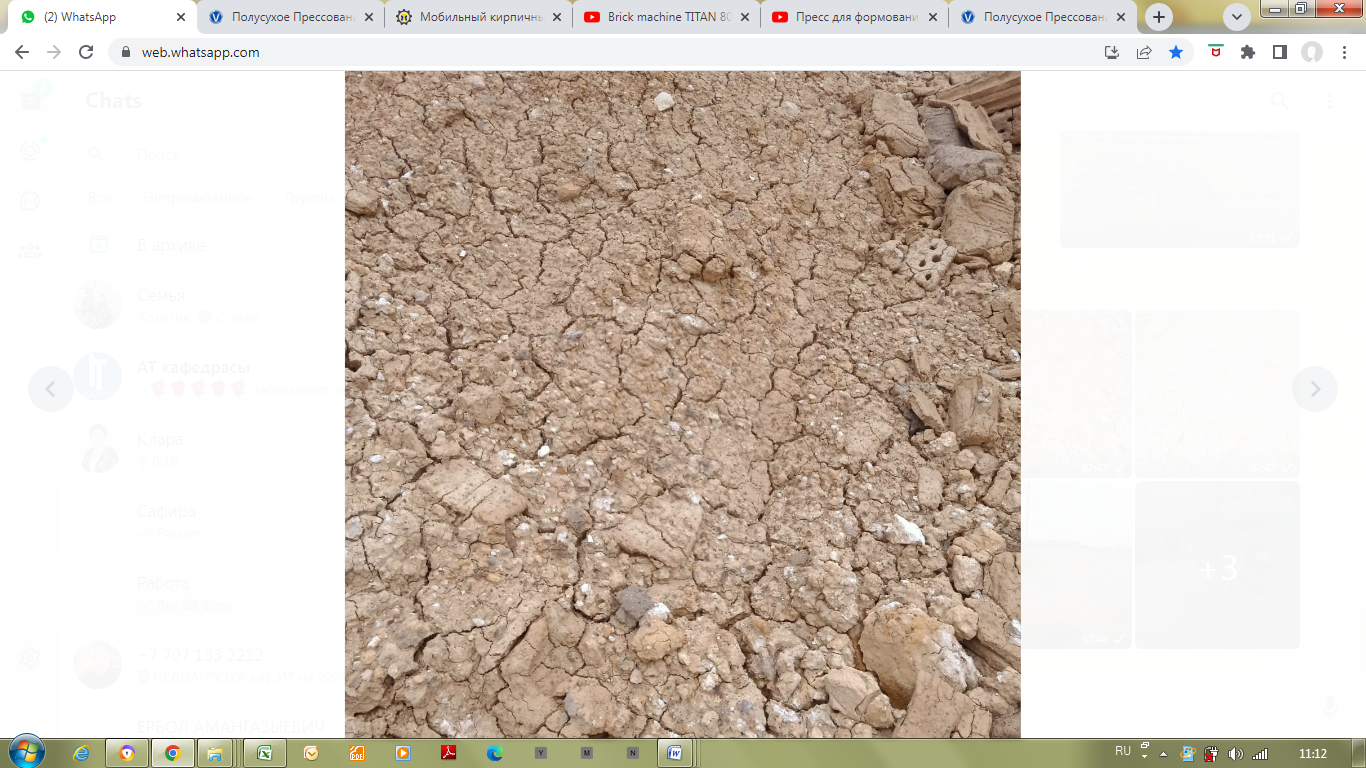
\includegraphics[width=\textwidth]{assets/266}
        \caption*{}
    \end{minipage}
    \hfill
    \begin{minipage}{0.43\textwidth}
        \centering
        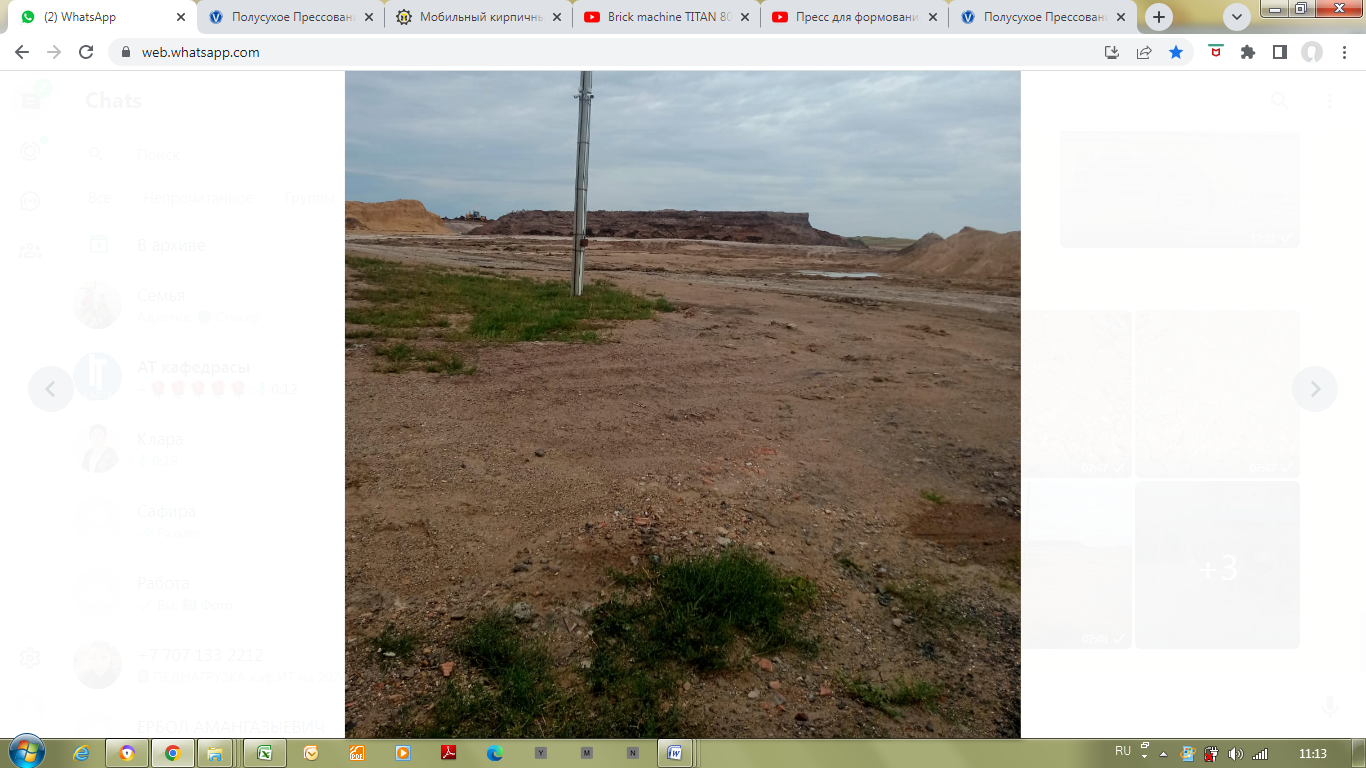
\includegraphics[width=\textwidth]{assets/267}
        \caption*{}
    \end{minipage}
	\caption*{\bfseries Figure 1 - Clay from the Ushkol quarry}
\end{figure}



\begin{figure}[H]
	\centering
	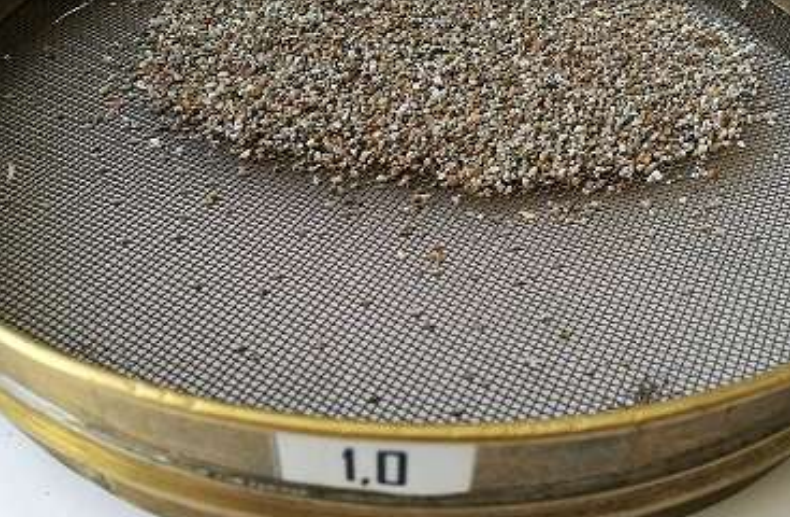
\includegraphics[width=0.5\textwidth]{assets/268}
	\caption*{\bfseries Figure 2 - Bauxite sludge (Pavlodar Aluminum Plant) fraction-1}
\end{figure}


\begin{figure}[H]
	\centering
	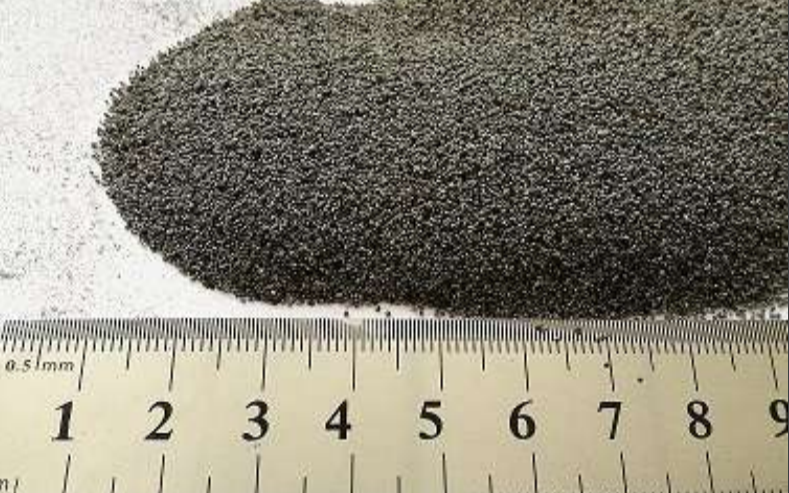
\includegraphics[width=0.5\textwidth]{assets/269}
	\caption*{\bfseries Figure 3 - Fly ash (Ekibastuz Gres -1) fraction-1}
\end{figure}



\begin{figure}[H]
	\centering
	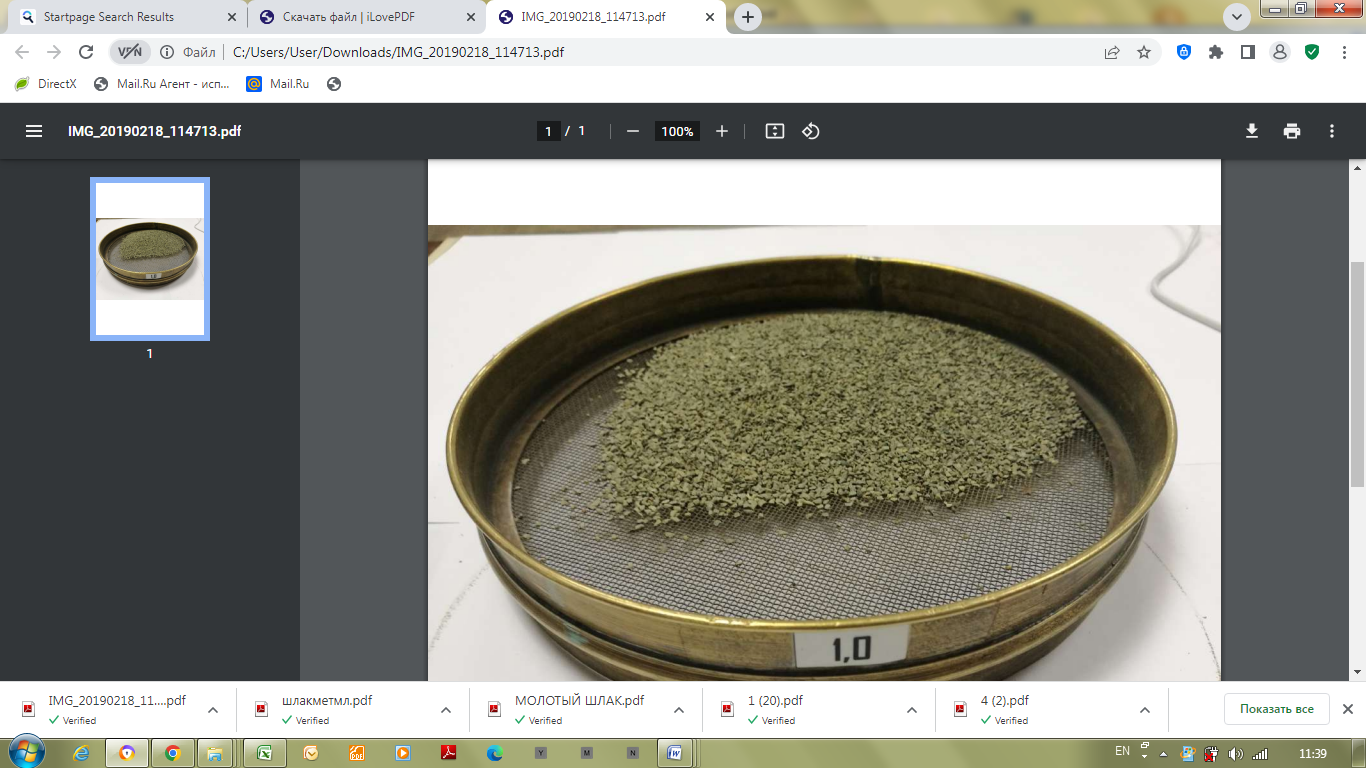
\includegraphics[width=0.5\textwidth]{assets/270}
	\caption*{\bfseries Figure 4−Metallurgical slag of Casting LLP fraction- 1}
\end{figure}



\begin{figure}[H]
	\centering
	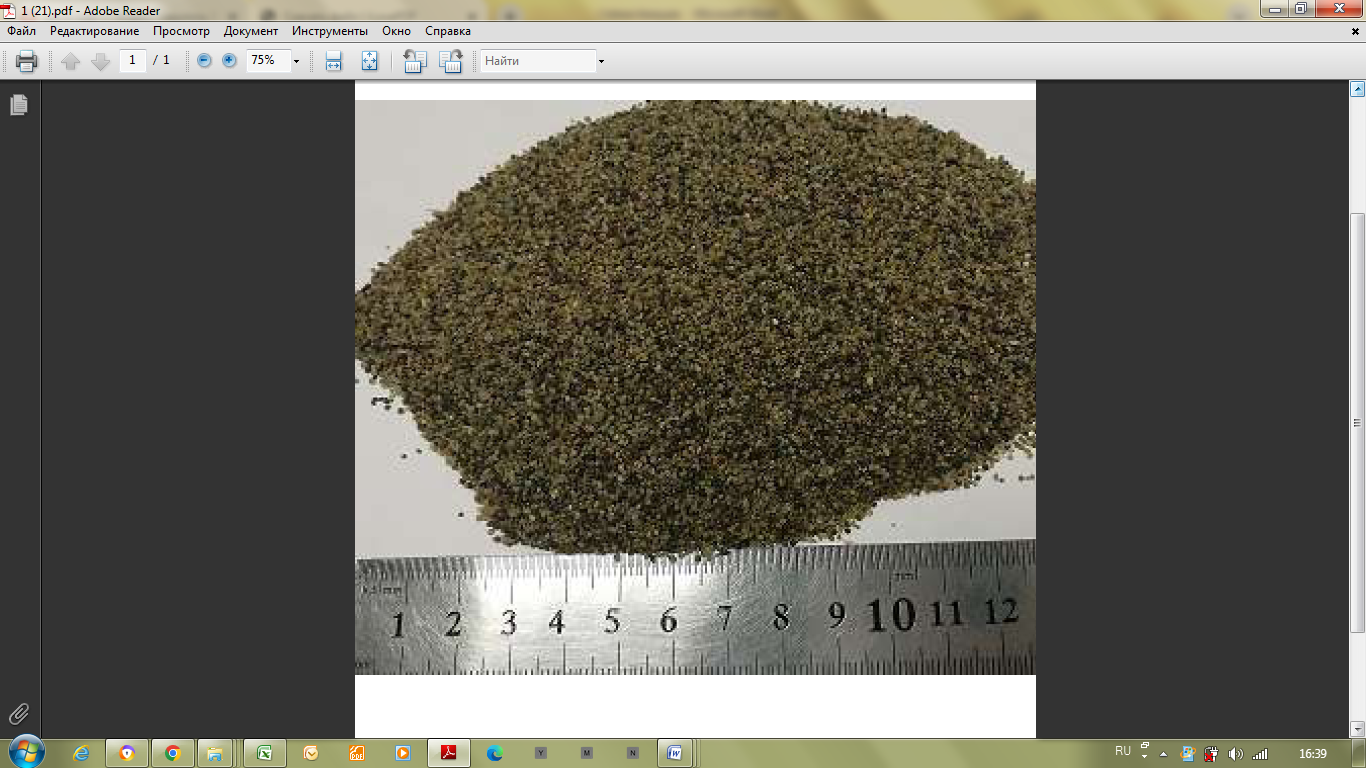
\includegraphics[width=0.5\textwidth]{assets/271}
	\caption*{\bfseries Figure 5 - River sand fraction- 1}
\end{figure}


\begin{multicols}{2}

The program allows you to simulate the operation of technological
equipment for the production of various construction products, including
ceramic ones.

Changes in the program related to the exclusion of the weight parameters
"cement", various additives that are not part of the raw materials for
the production of ceramic products, as well as the inclusion of the
parameter "clay" ensure that the model approximates the real
technological process. {[}6{]}. The algorithm of the program is
described in detail in {[}7{]}.

Listing 1 shows a fragment of a program for calculating the productivity
of technological equipment for the production of ceramic products based
on man-made raw materials.
\end{multicols}

\begin{lstlisting}
	float Norm(float, float);
	float ST[4];// list of events:
	// ST[0]-  the end of the mixture formation by the z0 device and transfer to mixing
	// ST[1]-  the end is mixing the mixture and pouring water z1
	// and transfer semi-dry to the molding matrix
	//  ST[2] – the end of the molding, the release of finished products z2
	//  ST[3]- simulation interval in min 8*60=480 - one shift
	Float Tt;// system time
	class OA0// service class. a device that forms a dry mixture
	{private:
	public:
	float Massa[NNp]; // the actual mass of the components of the mixture, case. value(+- dispenser error)
	int ne;// the current number of the container to which the OA is connected, ne =0.1,...4
\end{lstlisting}
\begin{multicols}{2}

When calculating the productivity of the technological line for the
production of ceramic products, the raw material "clay" was used, the
class OA1 was changed accordingly.
\end{multicols}

Listing 2 Class OA1 description program.

\begin{lstlisting}

	class OA1 // class-a maintenance apparatus that feeds clay and mixes
	{ private:
	 // Parameters OA:
	public:
	float tmixed;// mixing time
	float dtmatrica;// the time of transfer of the mixture to the matrix
	int sost;// 0- he is free and can take the mixture
				// 1 - the dry components have been transferred, the device is busy adding
				// add the clay to the mixture and mix before transferring the mixture
				// to the bunker, ordered the end time of the transfer
				// 2- simple, because it cannot transmit the mixture - the trace. OA is busy
				// 3 – simple, because no, the ingredient has run out (there is nothing to serve)
		//float massat; // the mass of the current charge transferred to the mixture.
	 Float summamass; // the mass of the dry mixture in OA transferred to the mixture.
	//float Sum;
	Float och;
	float proisv;
	float gen1();
	OA1();
	Int Fobr();
	Void display();
	   };
	
\end{lstlisting}

Class OA2 ensures the formation of ceramic products.

Listing 3 Class description program OA2.

\begin{lstlisting}

	class OA2  // The class is a service device that presses the mixture and delivers the finished product
	{ private:
	   // float massat; // the mass of the current mixture transferred to the molding matrix
	 public:
	float dtproduction;// time of transfer of finished products
	 int sost;// 0- he is free and can take a ready-made mixture
				// 1 - I am busy with the transfer of finished products and ordered the transfer time
	Float Sum;
	Float vmatr; // the volume of the matrix, kg
	 Int ki; // the number of products in the matrix
	 Float summamass; // the mass of the mixture in ОАО
	Float vsego;// total mass of products
		OA2();
	Float och;
	Float gen();//Working cycle time
	Void Fobr();//processing function
	Void display();
	  };
	OA0 z0;
	   OA1 z1;
	   OA2 z2;
	

\end{lstlisting}

\begin{lstlisting}

	Float MassaKomp[NNp];
	Float MassaKompSklad[NNp];
	 // NNp=0- Clay, NNp=1-sand,NNp=2 - no, NNp=3- ash
	//  NNp=4- metallurgical slag,  NNp=5-no,  NNp=6- bauxite sludge 
	 //  NNp=7 - no NNp=8 - no
	Float smes[NNp]; // the percentage composition of the mixture
	float MassaSmesy;// the planned total mass of the mixture,quantum, indivisible portion
	float vsmes;// The volume of the mixer with the finished mixture
	float massaprodution;
	
\end{lstlisting}


\begin{figure}[H]
	\centering
	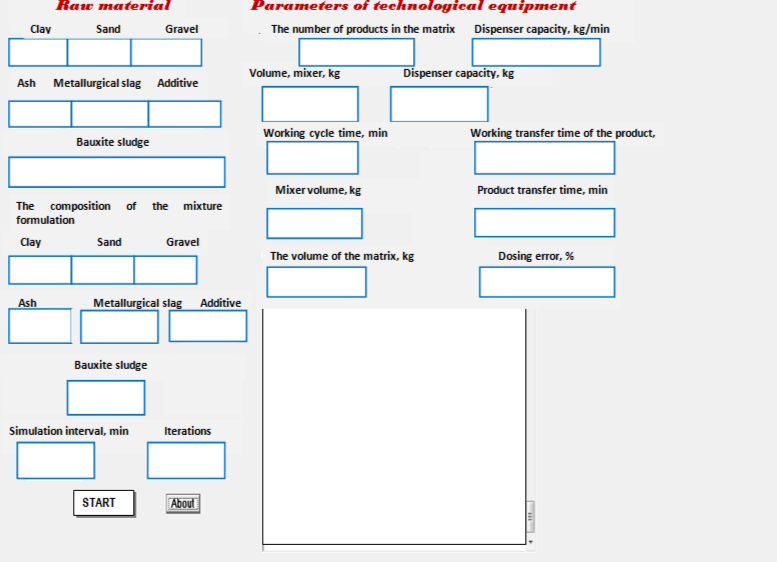
\includegraphics[width=0.55\textwidth]{assets/272}
	\caption*{\bfseries Figure 6 - Menu of the program for calculating the productivity of technological equipment for the production of ceramic
	products with additives of man-made raw materials}
\end{figure}



\begin{multicols}{2}
Fig. 6 shows the program menu for calculating the productivity of
technological equipment for the production of ceramic products with
additives of man-made raw materials.

The program menu shows 4 main parts:

1-raw materials in the warehouse of the enterprise;

2-the formulation of a mixture for the production of ceramic products,
makes it possible to simulate production with various additives and
volumes of artificial raw materials;

3-changing the parameters allows you to present the real picture of the
technological process as adequately as possible, in a digital display of
technical characteristics;

4-the simulation interval will allow you to calculate the performance of
technological equipment most accurately by setting any number of
iterations.

As it was presented above, a semi-dry production method was used in the
study, it is assumed that the humidity of the mixture is 6-7\%, while
additional equipment for drying products is not required.

Technological equipment for calculating productivity is represented by
Titanium 900-120DH EXpress brands Fig.7.
\end{multicols}

\begin{figure}[H]
	\centering
	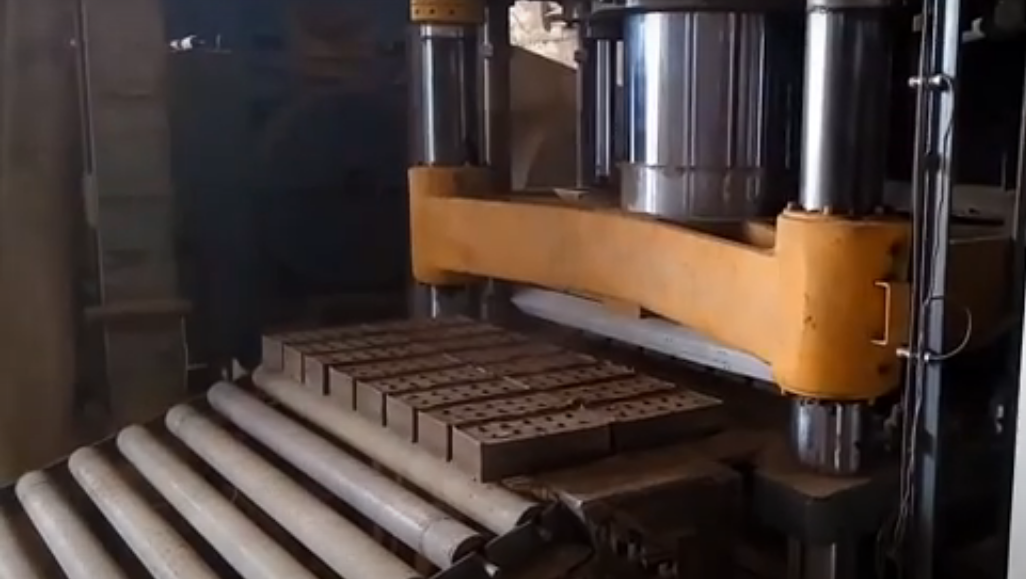
\includegraphics[width=0.5\textwidth]{assets/273}
	\caption*{\bfseries Figure 7 - Titanium Press 900-120 DHEX}
\end{figure}



\begin{figure}[H]
    \centering
    \begin{minipage}{0.49\textwidth}
		\centering
		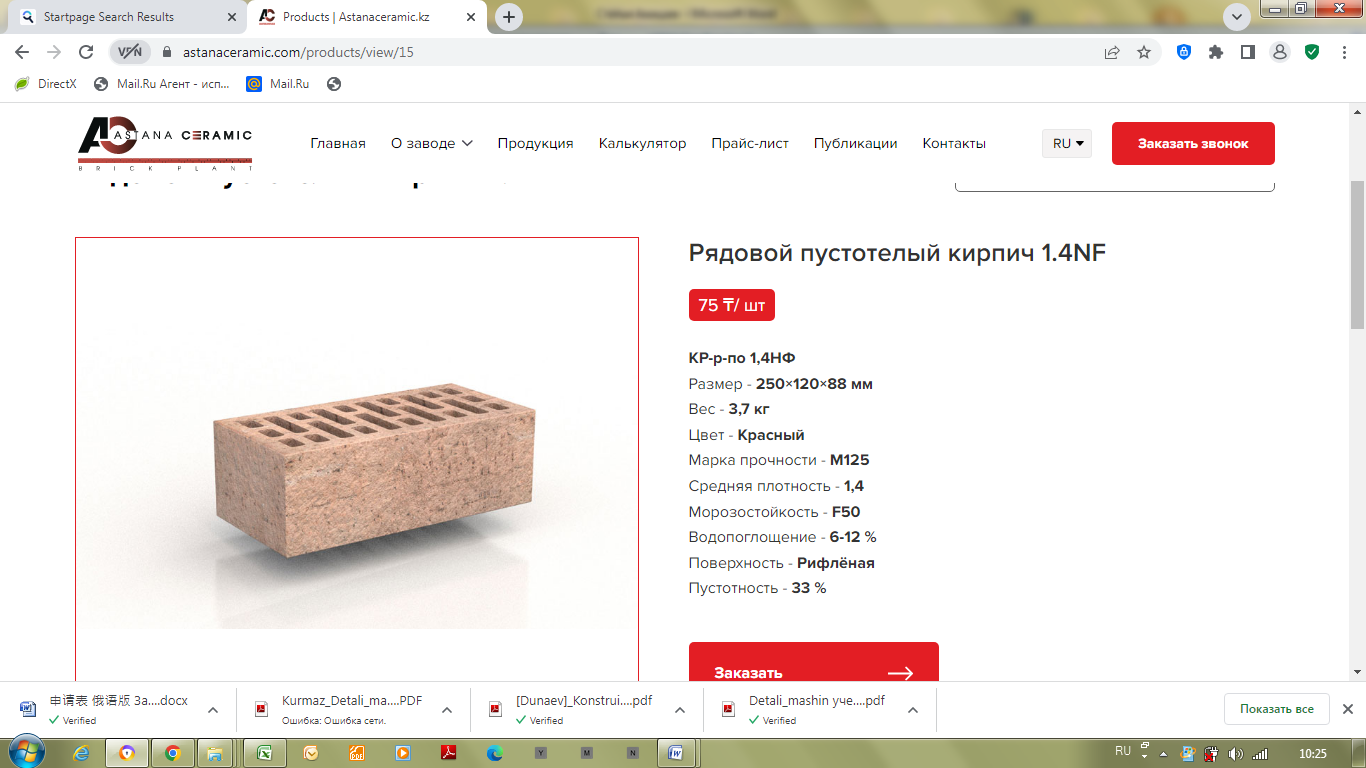
\includegraphics[width=\textwidth]{assets/274}
		\caption*{\bfseries Figure 8 - Ordinary hollow ceramic brick}
    \end{minipage}
    \hfill
    \begin{minipage}{0.49\textwidth}
		\centering
		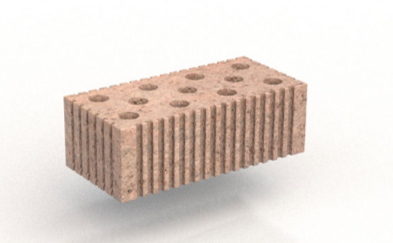
\includegraphics[width=\textwidth]{assets/275}
		\caption*{\bfseries Figure 9 - Ordinary full-bodied ceramic brick}
    \end{minipage}
\end{figure}

\begin{multicols}{2}


Let\textquotesingle s calculate the productivity for 2 types of ceramic
products, fig.8,9.

The technical characteristics of the processing line are indicated in
the passport of the Titanium 900-120 hexagonal press :

The duration of the working cycle is 11-12 minutes;

The drive power is 90 kW.

The number of products is 16 pcs.

The weight of the product is 3.7 kg and 4.3 kg (calculated taking into
account the additives of artificial raw materials).

The results of calculating the performance of the Titanium 900-120
hexagonal press are shown in Fig. 10;11.
\end{multicols}


\begin{figure}[H]
	\centering
	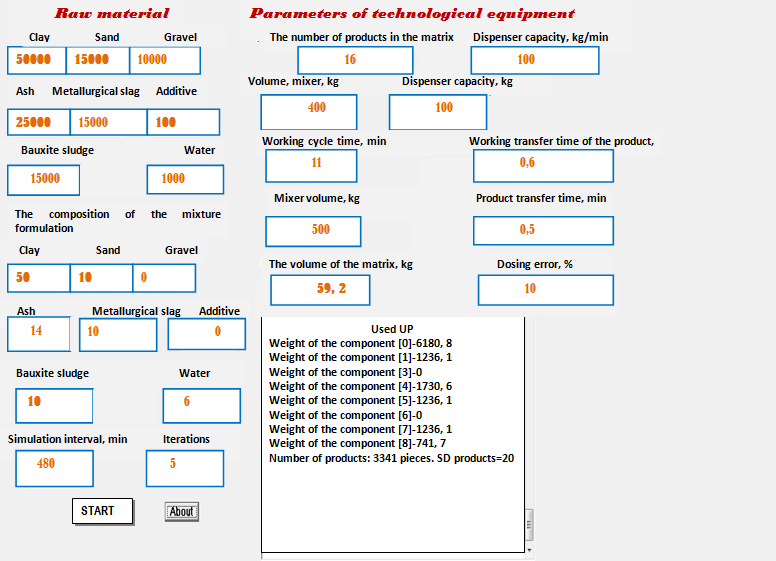
\includegraphics[width=0.65\textwidth]{assets/276}
	\caption*{\bfseries Figure 10 - Calculation of the productivity of technological
	equipment in the production of ordinary hollow ceramic bricks}
\end{figure}



\begin{figure}[H]
	\centering
	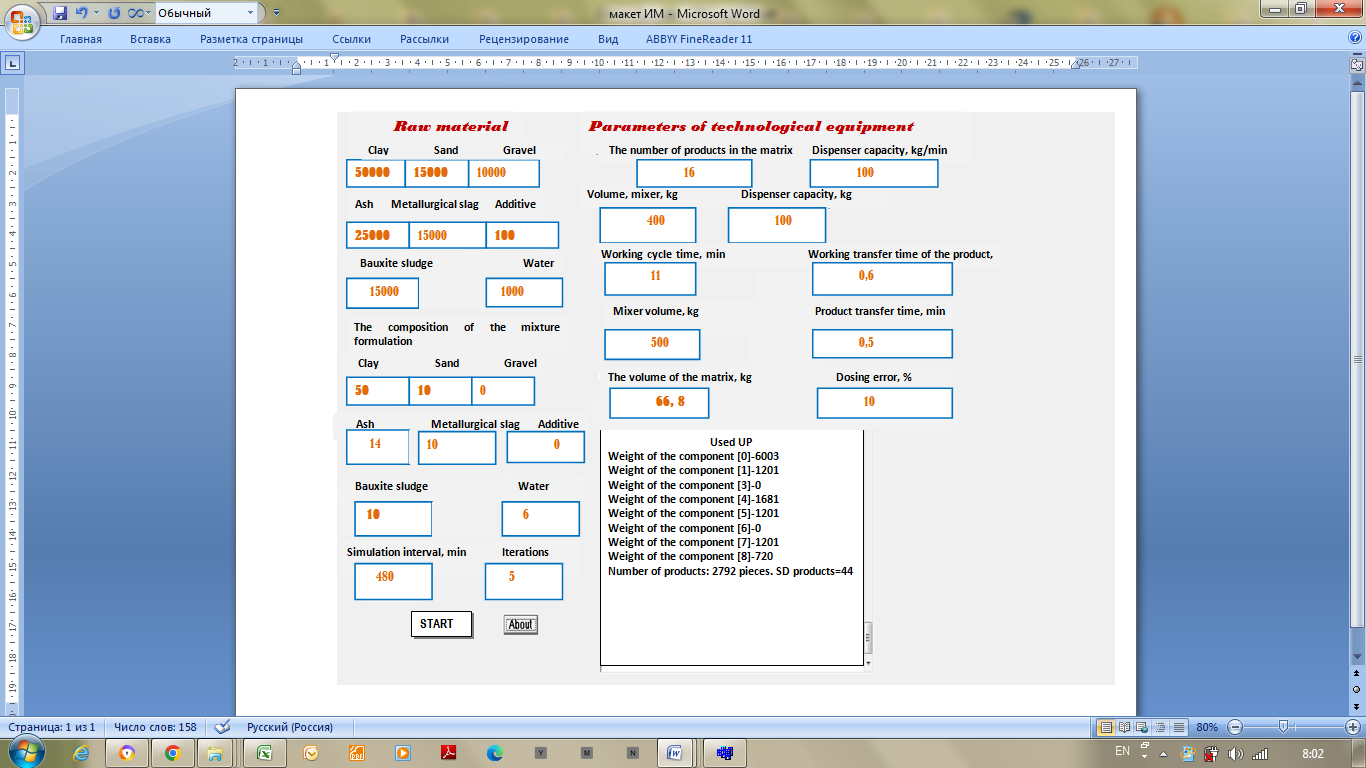
\includegraphics[width=0.65\textwidth]{assets/277}
	\caption*{\bfseries Figure 11−Calculation of the productivity of technological
	equipment in the production of ordinary full-bodied ceramic bricks}
\end{figure}



\begin{figure}[H]
	\centering
	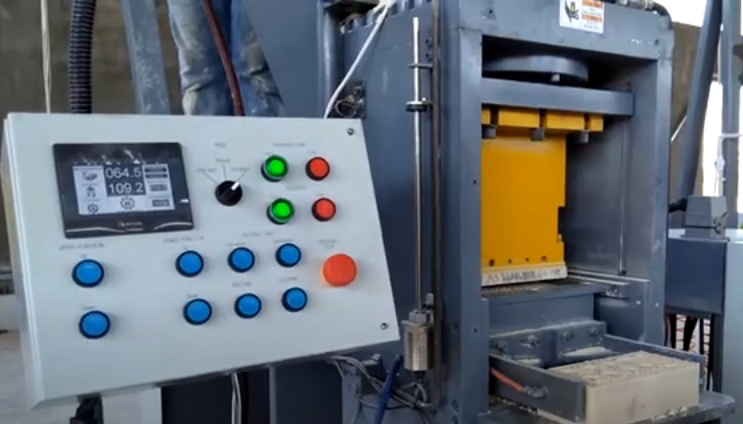
\includegraphics[width=0.66\textwidth]{assets/278}
	\caption*{\bfseries Figure 12 - Titanium 80 D Press}
\end{figure}

\begin{multicols}{2}


Similar calculations of the performance of technological equipment are
calculated by the program for the Titanium 80D press fig.12.

The technical characteristics of the processing line are given in the
passport of the Titanium 80D press:

The duration of the working cycle is 2-3 minutes;

The drive power is 15 kW.

The number of products is 1 pc.

The calculation of the productivity of the Titanium 80D press for two
types of ceramic bricks is shown in Fig. 13;14.
\end{multicols}

\begin{figure}[H]
	\centering
	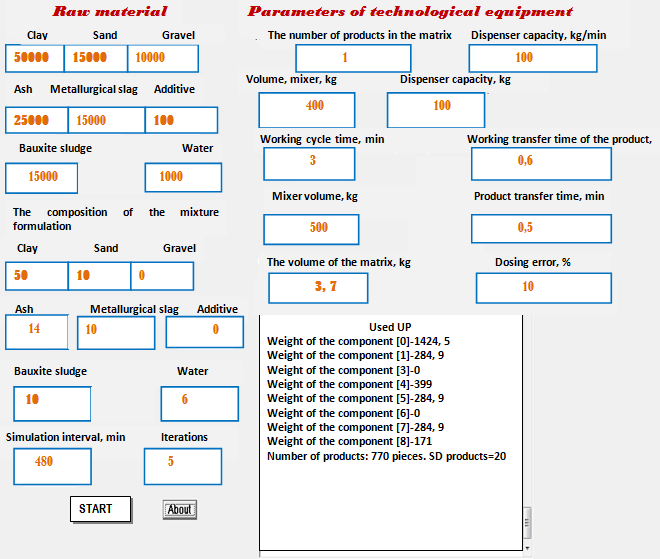
\includegraphics[width=0.6\textwidth]{assets/279}
	\caption*{\bfseries Figure 13 - Calculation of the productivity of technological
	equipment in the production  of ordinary hollow ceramic bricks}
\end{figure}



\begin{figure}[H]
	\centering
	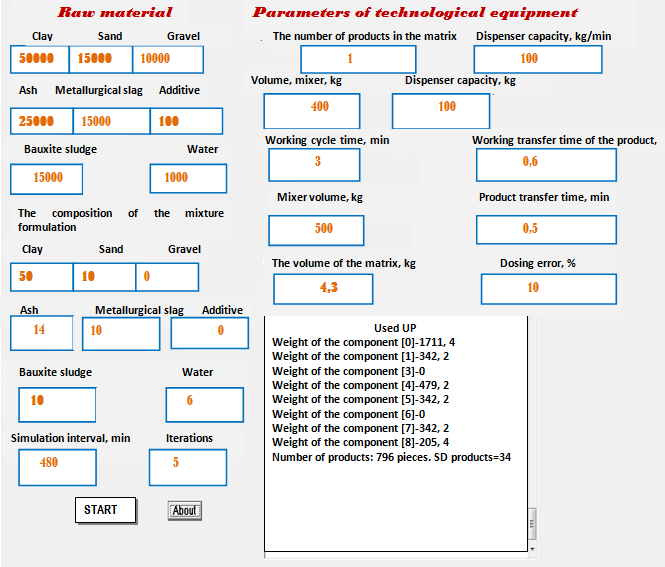
\includegraphics[width=0.6\textwidth]{assets/280}
	\caption*{\bfseries Figure 14−Calculation of the productivity of technological
	equipment in the production of ordinary full-bodied ceramic bricks}
\end{figure}

\begin{multicols}{2}


{\bfseries Conclusion.} The developed program allows you to:

1) perform calculations of the productivity of technological equipment
for semi-dry and dry methods of forming ceramic products, for various
types of molding matrices;

2) provides an opportunity to control the volume of raw materials in the
warehouse;

3) determine the calendar plan for the production of ceramic products;

4) flexibly respond to changes in the technological parameters of the
production process.

The program can be useful both for technologists of enterprises
producing construction products, and for individual entrepreneurs with a
limited number of technological equipment and a small volume of
production.

Existing developments related to simulation modeling are mainly related
to solving logistical problems, describing components and strategies,
and discrete events in particular {[}8-10{]}, which today opens up the
possibility of wider use of all information technology capabilities for
the practical implementation of engineering calculation tasks.
\end{multicols}


\begin{center}
	{\bfseries References}
	\end{center}

\begin{noparindent}

1.Glini dlya proizvodstva vyazhyshikh materialov.Tekhnicheskie ysloviya
{[}Clays for the production of binders Technical conditions{]}
{[}Electronic resource{]} {[}Access code{]}:URL:
https://online.zakon.kz/ Document/
?doc\_id=36318361\&pos=3;-106\#pos=3;-106 {[}in Russian{]}

2. Ob'em proizvodstva stroi materialov v Kazakhstane viros na 38,7\% za
devyat' mesyacev {[}The volume of construction materials production in
Kazakhstan increased by 38.7\% in nine months{]} {[}Electronic
resource{]} {[}Access code{]}: URL:~
https://qazindustry.gov.kz/anketa/article/1974-obem-proizvodstva-stroymaterialov-v-kazakhstane-vyros-na-387-za-devyat-mesyatsev
{[}in Russian{]}

3 Polysykhoe pressovanie keramicheskogo kirpicha.{[}Semi-dry pressing of
ceramic bricks{]} {[}Electronic resource{]} {[}Access code{]}:URL:
https://www.vgpress.ru/polusuhoe-pressovanie-kirpicha/ {[}in Russian{]}

4. Tekhnologiya proizvodstva kirpicha.{[} Brick production technology{]}
{[}Electronic resource{]} {[}Access code{]}\\URL:
https://keramikprof.ru/tehnologiya-proizvodstva-kirpicha/ {[}in
Russian{]}

5 Akishev K. Programma dlya EVM «Imitacionnaya model tekhnologicheskoi
linii proizvodstva stroitelnikh izdelii s ispolzovaniem otkhodov
promishlennogo proizvodstva».Svidetelstvo o vnesenii svedenii v
\\gosydarstvennii reestr prav na ob'ekti, okhranyaemie avtorskim
pravom.{[} The program for "Simulation model of a technological line for
the production of construction products using industrial waste".
Certificate of entry of information into the state register of rights to
objects protected by copyright.{]} №6653 от 26.11.2019

6. Akishev K and other. Mathematical formulation and the problem
solution of clustering recipes of concrete mixtures using technogenic
waste and slags of metallurgical enterprises.
\emph{Metalurgija}.-~2022.-61(1).-P.213--216.
https://www.scopus.com/authid/detail.uri?authorId=57267522000

7. Akishev.K., and other. Monografiya. Inzhernoe modelirovanie slozhnikh
tekhnologicheskikh sistem (proizvodstvo stroitelnikh izdelii s
ispolzovaniem tekhnogennikh otkhodov). {[}Monograph. Engineering
modeling of complex technological systems (production of construction
products using man-made waste).{]} Lantar-Books Publishing House,
Almaty, 2023.-142с, 500 inst. ISBN 978-601-361-254-6.
\\http://lantarbooks.kz/ru/shop/inzhenernoe-modelirovanie-slozhnyh-tehnologicheskih-sistem-proizvodstvo-stroitel-nyh-izdeliy-s-ispol-zo-\/-vaniem-tehnogennyh-othodov-monografiya

8. Kamil Szczesny. Adjusted recombination operator for simulation based
construction schedule \\optimization {[}Теxt{]}/ Szczesny Kamil //
Proceedings of the 2012 Winter Simulation Conference. -P.
652-661.997788-\/-11-\/-44667733-\/-44778802-\/-28//1122//©2012 IEEE.
https://informs-sim.org/wsc12papers/\\includes/files/inv158.pdf

9. Basnet. C. B. Experiences in developing an object-oriented modeling
environment for manufacturing systems {[}Теxt{]}/ C. B. Basnet //
Proceedings of the 1990 Winter Simulation Conference. -P. 477-481.
https://ieeexplore.ieee.org/document/129563

10. Preston K, Ricki J. The basics of simulation {[}Теxtт{]}/ K.
Preston, J/ Ricki // Proceedings of the 2016 Winter Simulation
Conference. -P.38-48/978-1-5090-4486-3/16 ©2016 IEEE.
https://informs-sim.org/\\wsc16papers/007.pdf
\end{noparindent}

\emph{{\bfseries Information about the authors}}
\begin{noparindent}

Akishev K. M. - Candidate of Technical Sciences, Ass. Professor, Kazakh
University of Technology and Business named after K. Kulazhanov, Astana,
Kazakhstan, e -mail:akmail04cx@mail.ru;

Aryngazin K.Sh.-Candidate of Technical Sciences, Professor, Director of
EcostroiNII-PV LLP, Pavlodar, Kazakhstan, kapar47@mail.ru;

Biybosynov B.I. -Doctor of Physical and Mathematical Sciences, Doctor
of Technical Sciences, Professor, Head of the Department of Applied
Mathematics and Computer Science of the I. Arabaev Kyrgyz State
University, Bishkek, Kyrgyzstan, bbolotbek@mail.ru;
\end{noparindent}

\emph{{\bfseries Информация об авторах}}
\begin{noparindent}

Акишев К. М. -к.т.н., асс. профессор, Казахский университет технологии и
бизнеса им. К. Кулажанова, Астана, Казахстан,e-mail:akmail04cx@mail.ru;

Арынгазин К.Ш.-к.т.н., профессор, директор ТОО «ЭкостройНИИ-ПВ», г.
Павлодар, Казахстан, \\kapar47@mail.ru;

Бийбосынов Б.И. -д.ф.м.н., д.т.н., профессор, заведующий кафедрой
«Прикладная математика и информатика» Кыргызского государственного
университета имени И. Арабаева., г. Бишкек, Кыргызстан,bbolotbek@mail.ru;
\end{noparindent}
